\chapter{Das Lebesgue-Maß}
  \begin{lemma}
    Der elementargeometrische Inhalt $vol^n: \script{Q}^n \to [0, \infty]$ ist ein Prämaß auf dem Halbring $\script{Q}^n$ im $\mathbb{R}^n$
  \end{lemma}

  \begin{proof}
    Sei $P = \bigcup\limits_{i=1}^{\infty}P_i$ mit $P_i \cap P_j = \varnothing$ für $i\neq j$, $P$,$P_i \in \script{Q}^n$ $\forall i\in \mathbb{N}$. \newline
    Satz II.27 (i.A. Satz II.26) $\implies vol^n$ ist Inhalt auf Ring $\script{F}^n  \implies \sum\limits_{i=1}^{\infty}vol^n(P_i)$ \newline $= \lim\limits_{k\to\infty}\sum\limits_{i=1}^{k}vol^n(P_i) = \lim\limits_{k\to\infty}vol^n(\bigcup\limits_{i=1}^{k}P_i) \leq vol^n(P)$. \newline
    Wähle zu $\epsilon > 0$ offene Quader $Q_i \supset P_i$ und einen kompakten Quader $Q \subset P$ mit $\sum\limits_{i=1}^{\infty}vol^n(Q_i) < \sum\limits_{i=1}^{\infty} vol^n(P_i) + \frac{\epsilon}{2}$, $vol^n(P)<vol^n(Q)+\frac{\epsilon}{2}$. \newline
    Satz von Heine-Borel (Satz (XIV).22 Ana1): $Q$ wird von endlich vielen Quadern \newline $Q_i\times ... \times Q_k$ überdeckt ($Q\subset P = \bigcup\limits_{i=1}^{\infty}P_i \subset  \bigcup\limits_{i=1}^{\infty}Q_i$) \newline $\implies vol^n(P) < vol^n(Q) +\frac{\epsilon}{2} \leq \sum\limits_{i=1}^{k}vol^n(Q_i) + \frac{\epsilon}{2} < \sum\limits_{i=1}^{\infty}vol^n(P_i)+\epsilon$. \newline
    Lasse $\epsilon > 0$ $\implies vol^n(P) \leq \sum\limits_{i=1}^{\infty}vol^n(P_i)$. 
  \end{proof}

  \begin{definition}
    Das \textbf{n-dimensionale äußere Lebesgue-Maß} einer Menge $E \subseteq \mathbb{R}^n$ ist definiert durch
    \begin{align*}
      \lambda^n(E) := inf\{\sum\limits_{k \in \mathbb{N}} vol^n(Q_k) \ | \ Q_k \in \script{Q}^n, E \subseteq \bigcup\limits_{k \in \mathbb{N}} Q_k\}
    \end{align*}
    $\lambda^n|_{\script{M}(\lambda^n)}$ ist das \textbf{n-dimensionale Lebesguemaß}.
  \end{definition}

  \begin{remark}
    Bem nach Satz II.31 (i.A. II.30) $\implies$ $\lambda^n$ regulär und vollständig auf $\script{M}(\lambda^n)$
  \end{remark}

  \begin{lemma}
    Betrachte für $k \in \mathbb{N}_0$ die Würfelfamilie $\script{W}_k = \{Q_{k,m} := 2^{-k}(m + [0,1]^n) \ | \ m \in \mathbb{R}^n\}$ und definiere für $E \subseteq \mathbb{R}^n$ die Mengen
    \begin{align*}
    F_k(E) := \bigcup \{Q \in \script{W}_k \ | \ Q \subseteq E\} \ \
    F^k(E) := \bigcup \{Q \in \script{W}_k \ | \ Q \cap E \neq \emptyset\}
    \end{align*}
    Dann gilt:
    \begin{enumerate}[label=\roman*)]
      \item $F_k(E)$ und $F^k(E)$ sind abgeschlossene Vereinigungen von abzählbar vielen kompakten Quadern mit paarweise disjunktem Inneren.
      \item $F_1(E) \subseteq F_2(E) \subseteq ... \subseteq E \subseteq ... \subseteq F^2(E) \subseteq F^1(E)$ 
      \item $F_k(E) \supseteq \{x \in \mathbb{R}^n \ | \ dist(x, \mathbb{R}^n \setminus E) > s^{-k} \sqrt{n}\}$\\
      $F^k(E) \subseteq \{x \in \mathbb{R}^n \ | \ dist(x, \mathbb{R}^n \setminus E) \leq s^{-k} \sqrt{n}\}$
      \item $\mathring{E} \subseteq \bigcup\limits_{k \in \mathbb{N}} F_k(E) \subseteq E \ \ \ , \ \ \ \bar{E} \supseteq \bigcap\limits_{k \in \mathbb{N}} F^k(E) \supseteq E$
    \end{enumerate}
  \end{lemma}

  \begin{proof}
    $\bigcup\{Q:Q\in W_k\} = \mathbb{R}^n$ $\forall k\in\mathbb{N}$. \newline
    $W_k$ hat abzählbar viele Elemente, die Würfel aus $W_k$ sind kompakt mit paarweise disjunktem Inneren und jede beschränkte Menge wird nur von endlich vielen Würfeln aus $W_k$ getroffen. $\implies F_k(E)$, $F^k(E)$ sind abgeschlossen $\implies$ i) \newline
    $Q_{k,m}$ ist Vereinigung der $2^n$ Teilwürfel $Q_{k+1, 2m+l}$ mit $l\in \{0,1\}^n$ und es gilt \newline $Q_{k,m} \subset E \implies Q_{k+1, 2m+l} \subset E$ $\forall l\in\{0,1\}^n$ \newline
    $Q_{k+1,2m+l} \cap E \neq \varnothing \implies Q_{k,m} \cap E \neq \varnothing$ wobei $l\in\{0,1\}^n$ \newline
    $\implies F_k(E) \subset F_{k+1}(E)$, $F^k(E) \supset F^{k+1}(E)$ $\implies$ ii) \newline
    Denn für $x \in E$ bel. existiert ein $Q\in W_k$ mit $x\in Q$. \newline
    Sei nun $x\in\mathbb{R}^n$ mit $dist(x,\mathbb{R}^n\setminus E) > 2^{-k}\sqrt{n} \implies \exists Q\in W_k$ mit $x\in Q$ und aus $dist(Q) = 2^{-k}\sqrt{n}$ folgt $Q\subset E \implies x\in F_k(E)\implies \{x\in\mathbb{R}^n: dist(x,\mathbb{R}^n\setminus E) > 2^{-k}\sqrt{n}\} \subset F_k(E)$. \newline
    Ist $x\in F^k(E) \implies \exists Q\in W_k$ mit $x\in Q$ und $Q \cap E \neq \varnothing \implies x\in F^k(E) \implies dist(x,E) \leq dist(Q) \leq 2^{-k}\sqrt{n} \implies$ iii) \newline
    iv) folgt sofort aus iii) und Def. von $\mathring{E}$ bzw. $\bar{E}$. 
    
  \end{proof}

  \sidenote{Vorlesung 9}{30.11.20}

  \begin{lemma}
    Die Borelmengen $\script{B}^n$ sind die vom Halbring $\script{Q}^n$ der Quader, dem Ring $\script{F}^n$ der Figuren, und dem System $\script{C}^n$ der abgeschlossenen Mengen des $\mathbb{R}^n$ erzeugten $\sigma$-Algebra, d.h. $\sigma(\script{Q}^n) = \script{B}^n = \sigma(\script{Q}^n) = \sigma(\script{F}^n) = \sigma(\script{C}^n)$
  \end{lemma}

  \begin{proof}
    siehe Aufschrieb
  \end{proof}

  \newpage
  \begin{theorem}
    Für $\lambda^n$ gilt:
    \begin{enumerate}
      \item Alle Borelmengen sind Lebesgue-messbar 
      \item Zu $E \subseteq \mathbb{R}^n \ \exists$ Borelmenge $B \supseteq E$ mit $\lambda^n(B) = \lambda^n(E)$
      \item $\lambda^n(K) < \infty \ \forall K \subseteq \mathbb{R}^n$ kompakt
    \end{enumerate}
  \end{theorem}

  \begin{proof}
    siehe Aufschrieb
  \end{proof}

  \begin{lemma}
    Für $E \subseteq \mathbb{R}^n$ beliebig gilt:
    \begin{enumerate}[label=\roman*)]
      \item $\lambda^n(E) = inf\{\lambda^n(U) \ | \ U \text{ offen }, U \supset E\}$
      \item $\lambda^n(E) = inf\{\lambda^n(K) \ | \ K \text{ kompakt }, K \subset E\}$, falls $E \ \lambda^n$-messbar
    \end{enumerate}
  \end{lemma}

  \begin{theorem}
    $D \subseteq \mathbb{R}^n$ ist genau dann $\lambda^n$-messbar, wenn eine der beiden Bedingungen gilt:
    \begin{enumerate}[label=\roman*)]
      \item $\exists$ Borlemenge $E \supset D$ mit $\lambda^n(E \setminus D) = 0$
      \item $\exists$ Borlemenge $C \subset D$ mit $\lambda^n(D \setminus C) = 0$
    \end{enumerate}
    Es kann $E = \bigcap\limits_{i \in \mathbb{N}} U_i$ mit $U_i$ offen und $C = \bigcup\limits_{j \in \mathbb{N}} A_j$ mit $A_j$ abgeschlossen gewählt werden.
  \end{theorem}

  \newpage

  \begin{theorem}[Satz von Lusin]
    Sei $A \subseteq \mathbb{R}^n$ offen mit $\lambda^n(A) < \infty$ und sei $f \ \lambda^n$-messbar auf $A$ mit Werten in $\mathbb{R}$. Dann existiert $\forall \epsilon > 0$ ein $K = K_{\epsilon} \subseteq A$ kompakt, mit:
    \begin{enumerate}[label=\roman*)]
      \item $\lambda^n(A \setminus K) < \epsilon$
      \item $f|_k$ ist stetig
    \end{enumerate}
  \end{theorem}

  \sidenote{Vorlesung 10}{4.12.20}

  \begin{definition}
    Ein äußeres Maß $\mu$ auf $\mathbb{R}^n$ heißt \textbf{Borelmaß}, falls gilt:
    \begin{enumerate}
      \item Alle Borelmengen sind $\mu$-messbar
      \item $\mu(K)<\infty \ \forall K \subseteq \mathbb{R}^n$ kompakt
    \end{enumerate}
  \end{definition}

  \begin{remark}
    $\lambda^n$ ist Borelmaß nach Satz III.5.\\
    Ein äußeres Maß $\mu$ auf $\mathbb{R}^n$ heißt \textbf{translationsinvariant}, falls \\
    $\mu(E + a) = \mu(E) \ \forall E \subset \mathbb{R}^n, a \in \mathbb{R}^n$ mit $E + a := \{x + a \ | \ x \in E\}$\\
    Bemerke: $vol^n:\script{Q}^n \to [0, \infty]$ ist translationsinvariant $\implies$ $\lambda^n$ ist translationsinvariant.
  \end{remark}

  \begin{lemma}
    Ist $\mu$ translationsinvariantes Borelmaß auf $\mathbb{R}^n$, so ist jede Koordinaten-Hyperebene $H := \{x \in \mathbb{R}^n \ | \ x_i = c\} (i=1,...,n)$ eine $\mu$-Nullmenge.
  \end{lemma}

  \begin{proof}
    siehe Aufschrieb
  \end{proof}

  \begin{theorem}
    Sei $\mu$ translationsinvariantes Borelmaß auf $\mathbb{R}^n$. Dann gilt mit $\theta := \mu([0,1]^n)$:
    \begin{align*}
      \mu(E) = \theta \lambda^n(E) \ \ \ \ \forall \ \lambda^n \text{-messbaren } E \subseteq \mathbb{R}^n
    \end{align*}
  \end{theorem}

  \begin{proof}
    siehe Aufschrieb
  \end{proof}

  \begin{lemma}
    $U \subseteq \mathbb{R}^n$ offen, $f: U \to \mathbb{R}^n$ lipschitz-stetig mit Konstante $\Lambda$ bzgl. $||.||_{\infty}$. Dann gilt:
    \begin{align*}
      \lambda^n(f(E)) \leq \Lambda^n \lambda^n(E) \ \ \ \ \forall E \subseteq U
    \end{align*}
  \end{lemma}

  \begin{proof}
    siehe Aufschrieb
  \end{proof}

  \begin{theorem}
    $U \subseteq \mathbb{R}^n$ offen und $f \in C^1(U, \mathbb{R}^n)$. Dann gilt:
    \begin{enumerate}
      \item $N \subseteq U$ $\lambda^n$-Nullmenge $\implies$ $f(N)$ $\lambda^n$-Nulllmenge
      \item $E \subseteq U$ $\lambda^n$-messbar $\implies$ $f(E)$ $\lambda^n$-messbar
    \end{enumerate}
  \end{theorem}

  \begin{proof}
    siehe Aufschrieb
  \end{proof}

  \begin{theorem}
    Sei $S \in O(\mathbb{R}^n)$ und $a \in \mathbb{R}^n$, dann gilt:
    \begin{align*}
      \lambda^n(S(E) + a) = \lambda^n(E) \ \ \ \ \forall E \subseteq \mathbb{R}^n
    \end{align*}
  \end{theorem}

  \begin{proof}
    siehe Aufschrieb
  \end{proof}

  \begin{lemma}[Polarzerlegung]
    $\forall S \in GL(\mathbb{R}^n) \ \exists$ Diagonalmatrix $\Lambda$ mit Einträgen $\lambda_i > 0, i=1,...,n$ und \\
    $T_1, T_2 \in O(\mathbb{R}^n)$, sodass $S = T_1 \Lambda T_2$ 
  \end{lemma}

  \begin{proof}
    siehe Aufschrieb
  \end{proof}

  \begin{theorem}[Lineare Transformationsformel]
    Für eine lineare Abbildung $S: \mathbb{R}^n \to \mathbb{R}^n$ gilt:
    \begin{align*}
      \lambda^n(S(E)) = |det(S)| \ \lambda^n(E) \ \ \ \ \forall E \subseteq \mathbb{R}^n
    \end{align*}
  \end{theorem}

  \begin{proof}
    siehe Aufschrieb
  \end{proof}

  \begin{example}
  \begin{minipage}{0.7\textwidth}
    $\lambda_1, ...,  \lambda_n > 0, \ E=\{x \in \mathbb{R}^n \ | \ (\dfrac{x_1}{\lambda_1})^2 + ... + (\dfrac{x_n}{\lambda_n})^2 < 1\}$\\
    mit $\Lambda = \begin{pmatrix}
      \lambda_1 & &\\
      & \ddots &\\
      & & \lambda_n
    \end{pmatrix}
    \in GL(\mathbb{R}^n)$ gilt $E = \Lambda(B_1(0))$\\
    Satz III.16 $\implies \lambda^n(E) = \lambda^n(\Lambda(B_1(0))) = \lambda_1 \cdot ... \cdot \lambda_n \cdot \lambda^n(B_1(0))$
  \end{minipage}\hfill
  \begin{minipage}{0.3\textwidth}
    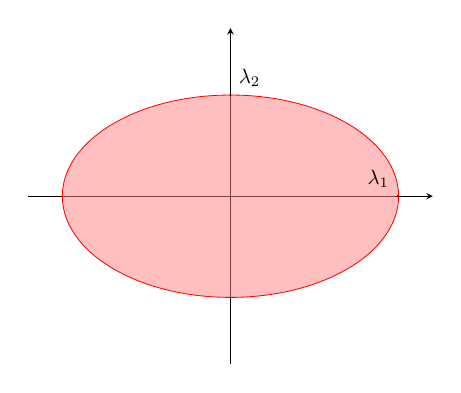
\begin{tikzpicture}[scale=.75]
      \begin{axis}[
        xmin=-2, xmax=2,
        ymin=-2, ymax=2,
        xtick=\empty,
        ytick=\empty,
        axis lines=middle,
        ]
        \draw[red, fill=red!50, fill opacity=0.5] (axis cs:0,0) ellipse [rotate=90, x radius=1, y radius=2];
        \node[label={45:{$\lambda_2$}},circle,fill,inner sep=0pt] at (axis cs:0,1.2) {};
        \node[label={135:{$\lambda_1$}},circle,fill,inner sep=0pt] at (axis cs:1.65,0) {};
      \end{axis}
    \end{tikzpicture}
  \end{minipage}
  \end{example}

  \begin{example}[Vitali 1905]
    $\script{P}(\mathbb{R}^n) \neq \script{M}(\lambda^n)$\\
    Beweis siehe Aufschrieb.
  \end{example}

  